\documentclass[a4paper,11pt]{article}
\usepackage{amsmath,amsthm,amsfonts,amssymb,amscd,amstext,vmargin,graphics,graphicx,tabularx,multicol} 
\usepackage[francais]{babel}
\usepackage[utf8]{inputenc}  
\usepackage[T1]{fontenc} 
\usepackage{pstricks-add,tikz,tkz-tab,variations}
\usepackage[autolanguage,np]{numprint} 
\usepackage{color}
\usepackage{ulem}

\setmarginsrb{1.5cm}{0.5cm}{1cm}{0.5cm}{0cm}{0cm}{0cm}{0cm} %Gauche, haut, droite, haut
\newcounter{numexo}
\newcommand{\exo}[1]{\stepcounter{numexo}\noindent{\bf Exercice~\thenumexo} : \marginpar{\hfill /#1}}
\reversemarginpar


\newcounter{enumtabi}
\newcounter{enumtaba}
\newcommand{\q}{\stepcounter{enumtabi} \theenumtabi.  }
\newcommand{\qa}{\stepcounter{enumtaba} (\alph{enumtaba}) }
\newcommand{\initq}{\setcounter{enumtabi}{0}}
\newcommand{\initqa}{\setcounter{enumtaba}{0}}

\newcommand{\be}{\begin{enumerate}}
\newcommand{\ee}{\end{enumerate}}
\newcommand{\bi}{\begin{itemize}}
\newcommand{\ei}{\end{itemize}}
\newcommand{\bp}{\begin{pspicture*}}
\newcommand{\ep}{\end{pspicture*}}
\newcommand{\bt}{\begin{tabular}}
\newcommand{\et}{\end{tabular}}
\renewcommand{\tabularxcolumn}[1]{>{\centering}m{#1}} %(colonne m{} centrée, au lieu de p par défault) 
\newcommand{\tnl}{\tabularnewline}

\newcommand{\bmul}[1]{\begin{multicols}{#1}}
\newcommand{\emul}{\end{multicols}}

\newcommand{\trait}{\noindent \rule{\linewidth}{0.2mm}}
\newcommand{\hs}[1]{\hspace{#1}}
\newcommand{\vs}[1]{\vspace{#1}}

\newcommand{\N}{\mathbb{N}}
\newcommand{\Z}{\mathbb{Z}}
\newcommand{\R}{\mathbb{R}}
\newcommand{\C}{\mathbb{C}}
\newcommand{\Dcal}{\mathcal{D}}
\newcommand{\Ccal}{\mathcal{C}}
\newcommand{\mc}{\mathcal}

\newcommand{\vect}[1]{\overrightarrow{#1}}
\newcommand{\ds}{\displaystyle}
\newcommand{\eq}{\quad \Leftrightarrow \quad}
\newcommand{\vecti}{\vec{\imath}}
\newcommand{\vectj}{\vec{\jmath}}
\newcommand{\Oij}{(O;\vec{\imath}, \vec{\jmath})}
\newcommand{\OIJ}{(O;I,J)}


\newcommand{\reponse}[1][1]{%
\multido{}{#1}{\makebox[\linewidth]{\rule[0pt]{0pt}{20pt}\dotfill}
}}

\newcommand{\titre}[5] 
% #1: titre #2: haut gauche #3: bas gauche #4: haut droite #5: bas droite
{
\noindent #2 \hfill #4 \\
#3 \hfill #5

\vspace{-1.6cm}

\begin{center}\rule{6cm}{0.5mm}\end{center}
\vspace{0.2cm}
\begin{center}{\large{\textbf{#1}}}\end{center}
\begin{center}\rule{6cm}{0.5mm}\end{center}
}



\begin{document}
\pagestyle{empty}
\titre{Interrogation: Les nombres entiers }{Nom :}{Prénom :}{Classe}{Date}


\exo{1} Compléter  les phrases suivantes :\\

\bi 
\item Un \textcolor{red}{nombre} est composé de chiffres.\\

\item 39 est un \textcolor{red}{nombre} composé de deux \textcolor{red}{chiffres}\\

\ei

\vspace*{0.6cm}

\exo{1} Écrire les nombres suivants en chiffres :\\


\q Soixante-douze mille cinquante : \textcolor{red}{72 050}\\

\q Seize millions cinq cent vingt-trois : \textcolor{red}{16 000 523}\\

\vspace*{0.6cm}

\exo{3} Compléter comme indiqué à la première ligne.

\begin{flushleft}
\includegraphics[scale=1]{tab1.eps} 
\end{flushleft}

\vspace*{0.6cm}

\exo{2}\\

\initq
\q Dans le nombre 450 019 237, quel est le chiffre des unités de milliards ?  \\
\textcolor{red}{Le chiffre des unités de milliards est 0.}\\

\q Dans le nombre 99 500 346, quel est le chiffre des centaines de mille ? \\
  \textcolor{red}{Le chiffre des centaines de mille est 5.}\\

\q Dans le nombre 36 041, quel est le nombre de dizaines ? \\ \textcolor{red}{Le nombre de dizaines est 3 604.} \\

\vspace*{0.6cm}

\exo{2} Ajouter des zéros (s'il en faut) pour que 5 soit le chiffre \textit{des dizaines de mille} de chaque nombre :\\

\textcolor{red}{97 850 000}	\hspace*{3cm}		\textcolor{red}{750 300}		\hspace*{3cm}		\textcolor{red}{251 039}	\hspace*{3cm}			\textcolor{red}{1 256 000}\\

\vspace*{0.6cm}

\exo{1} Dire si les nombres suivants sont égaux (=) ou différents ($ \ne$ )\\

	  405 \textcolor{red}{ = }  0405      \hspace*{3cm}                 10 571 \textcolor{red}{ $ \ne$ }  1 571










\end{document}


